\documentclass[a4paper, 12pt]{article}
\usepackage[utf8]{inputenc}
\usepackage{geometry}
\usepackage{polski}
\usepackage{graphicx}
\usepackage{float}
\usepackage{etoolbox,refcount}
\usepackage{multicol}

\newgeometry{left=2cm, right=2cm, bottom=2cm, top=1.5cm}

\begin{document}
	\begin{figure}[H]
		\centering
		\includegraphics[height=6cm, width=\textwidth]{./img/lena.png}
	\end{figure}
	\section{Cel ćwiczenia}
		Celem ćwiczenia laboratoryjnego jest nabycie umiejętności programowania prostego, jednokanałowego regulatora, którego zadaniem w ćwiczeniu jest sterowanie temperaturą, jednak może być wykorzystany również do regulacji innych wielkości przetworzonych na sygnał standardowy w niewielkich instalacjach. Kolejnym celem jest zapoznanie się ze sposobami pomiaru temperatury oraz schematami regulacji procesów temperaturowych oraz nauczenie się obsługiwania skrajnie minimalistycznych interfejsów użytkownika. 
	\section{Schemat układu}
		\begin{figure}[H]
			\centering
			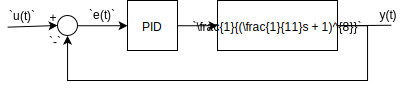
\includegraphics[width=\textwidth]{./img/schemat.png}
			\caption{Schemat połączeń układu regulacji}
		\end{figure}
		Układ pomiarowy składa się z dwóch termometrów platynowych Pt100, zamontowanych symetrycznie do siebie. Obydwa termometry są połączone w systemie trójprzewodowym (najczęściej stosowanym, z częściową kompensacją). Jeden z nich jest połączony z wejściem regulatora,\linebreak a drugi z gniazdami na przedniej ścianie obudowy. Badają one temperaturę obiektu regulacji, jakim jest walec aluminiowy zamocowany we wkładzie grzejnym do lutownicy o mocy 400 W. Spirala grzejna jest zasilana impulsowo z wyjścia regulatora sygnałem sieciowym 220 V. \linebreak W prawej ścianie obudowy jest wbudowany wentylator uruchamiany z wyjścia alarmowego AL1 regulatora, stosowany do chłodzenia w przypadkach przekroczenia wartości zadanej. Sterowanie sygnałami sieciowymi jest przeprowadzane przy pomocy PWM (Pulse Width Modulation), która polega na modulacji współczynnika wypełnienia sygnału sterującego. Aby ułatwić chłodzenie obiektu regulacji ma on pokarbowane wystające końce.
	\section{Termometr platynowy w układzie trójprzewodowym}
		Termometr Pt100 jest w przypadku z ćwiczenia połączony jednym z najczęściej stosowanych połączeń - połączeniem trójprzewodowym. Jest ono łączone z mostkiem Whetsotne'a i służy do wyeliminowania oporu przewodu, zwiększając tym samym dokładność pomiarów i zmniejszając potencjalne zakłócenia, gdyż zmiany oporności oddziałują w tym przypadku symetrycznie na opór obwodów elektrycznych (pomiarowego i porównawczego). 
		\newline
		\newline
		Oznaczenia termometru rezystancyjnego oznaczają, że jest on wykonany z platyny i, że\linebreak w temperaturze $0^oC$ posiada rezystancję $100 \ \mathrm{\Omega}$. Jest to bardzo często stosowany termometr rezystancyjny, który w atmosferze obojętnej może może być stosowany do 1000 $^o$C, jednak najczęstszym zakresem jego stosowania jest zakres od -220 do 850 $^o$C. Jest szeroko stosowany ze względu na swoją liniowość w dużym zakresie temperatur. 
	\section{Regulator RE31}
		Regulator został zaprojektowany aby zabezpieczyć go przed przypadkowymi zmianami wartości ustawianych przez użytkownika. Aby osiągnąć to, menu zostało podzielone na trzy poziomy dostępu w zależności od częstości zapotrzebowania na dane ustawienia. Dlatego też wartości jakie podajemy najczęściej, czyli wartości alarmów i wartość zadana są najwyżej w hierarchii. Dalej znajdują się rzadziej zmieniane nastawy regulatora takie jak czas całkowania, czas różniczkowania, zakres proporcjonalności lub chociażby ustawienia histerezy. Najniżej w hierarchii są najrzadziej zmieniane nastawy, takie jak typy alarmów czy jednostka temperatury.
		\newline 
		\newline
		Poruszanie się w ustawieniach regulatora odbywało się przy pomocy najbardziej wysuniętego na lewo przycisku, który w przypadku jednorazowego naciśnięcia odpowiadał za przełączanie się między opcjami z danego poziomu, a dłuższe przytrzymanie go po osiągnięciu ostatniej opcji danego poziomu przechodzi do kolejnego poziomu. Jedną z ciekawszych funkcji regulatora Re31 jest opcja samostrojenia się w zależności od potrzeb - jednak ze względu na czas jej trwania nie jest ona pokryta przez program ćwiczenia.
	\section{Przebieg ćwiczenia}
		Ćwiczenie rozpoczęliśmy od ustawienia odpowiednich parametrów regulatora: 
		\begin{itemize}
			\item Typ wejścia: Pt100 JS
			\item Dolna granica zakresu: $10^o\mathrm{C}$
			\item Górna granica zakresu: $300^o\mathrm{C}$
			\item Dolne ograniczenie mocy wyjściowej: 0\%
			\item Górne ograniczenie mocy wyjściowej: 100\%
			\item Wartości zadane: $100^o\mathrm{C}$ oraz $200^o\mathrm{C}$
			\item Alarm A1: względny($+2^o\mathrm{C}$, $+10^o\mathrm{C}$, $+50^o\mathrm{C}$), bezwzględny($+2^o\mathrm{C}$, $+10^o\mathrm{C}$, $+50^o\mathrm{C}$)
			\item Rodzaj regulacji: inwersyjne
		\end{itemize}
		Ćwiczenie składało się z dwóch cżęści:
		\subsection{Regulator dwupołożeniowy}
			Pierwszą częścią ćwiczenia było zbadanie pracy regulatora w trybie regulacji dwupołożeniowej dla różnych wartości histerezy. Do przejścia w ten tryb musieliśmy ustawić wartość zakresu proporcjonalności Pb na 0. 
			\newline
			\newline
			Rozpoczęliśmy od zbadania dla wartości zadanej równej 100 $^o$C, z włączoną histerezą 1 $^o$C i alarmem względnym na poziomie +2 $^o$C Grzałka została włączona przy temperaturze 99,2 $^o$C i wyłączyła się w temperaturze 101,1 $^o$C. Wartość maksymalna temperatury wynosiła dla tego przebiegu 110 $^o$C. 
			\newline
			\newline 
			Następnie zwiększyliśmy parametry histerezy do wartości 2 $^o$C, aby zbadać zależność amplitudy oscylacji od histerezy. Grzanie zostało włączone przy temperaturze 98,9 $^o$C, a wyłączone przy temperaturze 102 $^o$C. Maksymalna temperatura wynosiła 112 $^o$C, a minimalna 98,6 $^o$C.
			\newline 
			\newline
			Następnie zwiększyliśmy temperaturę do wartości zadanej 200 $^o$C. Histerezę ustawiliśmy na 2 $^o$C, a alarm względny na 10 $^o$C.  Włączenie grazłki następowało przy temperaturze 198,5 $^o$C, a jej wyłączanie przy temperaturze 202 $^o$C. Przy temperaturze 210 $^o$C załączał się alarm. Maksymalna temperatura wyniosła 213 $^o$C.
		\subsection{Regulator PID} 
			Drugą częścią ćwiczenia było zaprogramowanie regulatora w trybie PID z wyjściem dwupołożeniowym, przyjmując poniższe nastawy regulatora:
			\begin{center}
				\begin{tabular}{|c|c|c|}
					\hline Nastawy/Wartość zadana & $100\ ^o$C & $200\ ^o$C  \\ 
					\hline $Pb \ [^o\mathrm{C}]$ & 40  & 16  \\ 
					\hline $T_i \ [\mathrm{s}]$ & 166 & 103 \\ 
					\hline $T_d \ [\mathrm{s}]$ & 209 & 51 \\ 
					\hline 
				\end{tabular} 
			\end{center}
			Praca regulatora PID przebiegała z okresem impulsowania równym 5s oraz alarmem AL1 względnym ustawionym na +10 $^o$C.
			\newline 
			\newline
			Przeprowadziliśmy pomiar dla temperatury 200 $^o$C i dla temperatury 100 $^o$C, przy okazji chłodząc układ. Oraz dokonując drobnych odchyłek, tak jak to jest zadane w treści ćwiczenia, obserwując przy tym jak działa modulacja PWM, którą można bardzo dobrze przy tych nastawach zaobserwować.
		\section{Obserwacje i wnioski}
			Po zachowaniu się obiektu regulacji można wywnioskować, że posiada on bardzo dużą inercję, a oprócz tego jest wystarczająco nieliniowy, aby przyjąć do strojenia regulatora PID dwa różne punkty pracy. Jeden z punktów pracy daje nastawy dla temperatury 100 $^o$C, a drugi daje nastawy dla temperatury 200 $^o$C. Bierze to się chociażby stąd, że moc promieniowania cieplnego jest zależna od czwartej potęgi temperatury w skali absolutnej oraz z tego, że energia jest efektywniej przekazywana między ośrodkami o większej różnicy temperatur (większy strumień).
			\newline
			\newline
			W trakcie ćwiczenia mogliśmy zaobserwować wpływ zwiększenia histerezy na amplitudę oscylacji wokół wartości przez nas zadanej. Zwiększenie histerezy generowało większe oscylacje, a co za tym idzie - większe przesterowania, co może być potencjalnie niebezpieczne dla niektórych zastosowań, w których nie można dopuścić do przedwczesnego przekroczenia pewnej wartości takich jak chociażby sterowanie zapłonem, gdzie przedwczesne przekroczenie pewnej wartości może doprowadzić do awarii albo nawet zniszczenia układu.
			\newline 
			\newline 
			W przypadku działania regulatora PID można było zauważyć realizację PWM, gdyż ten raz na jakiś czas włączał grzałkę aby następnie ją wyłączyć po chwili. Było to szczególnie widoczne jak przełączaliśmy sterowanie PID z wartości 200 $^o$C na 100 $^o$C, a grzałka grzała pełną mocą przez pewien czas, pomimo dużej różnicy między wartością zadaną, a aktualnie odczytaną\linebreak z aparatury. Ponieważ nagrzewanie powodowało zmianę kąta nachylenia funkcji, którą wychwytywał człon różniczkujący, co mogło powodować dłuższe studzenie się mechanizmu.
			\newline 
			\newline 
			Zastosowanie regulatorów dwupołożeniowych ze względu na zaobserwowaną przez nas tendencję do przeregulowań nie sprawdzają się do wielu zagadnień, które wymagają precyzji. Nawet niewielka histereza sprawia, że ciągle będziemy oscylować wokół zadanej wartości, jednak nigdy się na niej nie stabilizując. Dodatkowo zwiększenie histerezy powoduje rzadsze przełączenia, co tylko zmniejsza dokładność takiego rozwiązania. 
			\newline 
			\newline
			Nie mniej jednak jest to dobre rozwiązanie chociażby w żelazkach lub płytach indukcyjnych, gdzie wahania kilku stopni lub polu elektromagnetycznym nie generują zbyt wielkiej różnicy\linebreak w wyniku końcowym, lub w sytuacjach, gdzie liczy się ograniczenie kosztów.
			\newline 
			\newline
			Ćwiczenie to nauczyło nas jak sobie radzić z minimalistycznym interfejsem użytkownika, gdyż bardziej rozbudowane opcje nie zawsze są dostępne ze względu na koszty i liczebność w jakiej występuje dane urządzenie. Czasami nie opłaca się wykonać większych paneli sterowania, albo są urządzenia są na to za małe. W takiej sytuacji nie ma często innej opcji niż skorzystać z minimalistycznego interfejsu w celu zaprogramowania regulatora, gdyż wyprowadzenia do przyrządów pomiarowych lub komputera są zbyt drogie w stosunku do reszty produktu albo warunki nie pozwalają do zastosowania ich.
\end{document}